\chapter{Experiments and Results}
\label{chap:ExperimentsAndResults}

TODO: quick chapter overview

\begin{code}
$ python3 main.py unet train --val_pages 123 ...
\end{code}


\section{Architecture}
\label{sec:Architecture}

In the \emph{generative model} approach to semi-supervised learning, one usually starts with a model that can be trained in the unsupervised manner (either an autoencoder or a generative adversarial network [CITE, CITE]) and then extends it to also perform the supervised task. For example, when starting with an autoencoder, one can use the encoder part as a dimensionality reduction mechanism and then build a supervised classification network that classifies the learned embeddings [CITE].

In our context of music recognition, we are highly motivated to build on top of the U-Net architecture [CITE] (figure \ref{fig:ArchitectureCombined}). It has first been used for biomedical image segmentation, however its superiority for object detection in music recognition has clearly been demonstrated by Pacha et al. [CITE].

The architecture can be viewed as a fully convolutional autoencoder with residual (skip) connections added between the encoder and decoder on every resolution level. The U-Net encoder is a typical fully-convolutional encoder that gradually reduces image dimensions, while increasing the channel count. Such an architecture is able to learn abstract representations of symbols present in the input image. The decoder then tries to go from these abstract representations back to specific ones, while at the same time modifying the reconstruction to fit the learned segmentation task. The core idea behind this architecture is that the decoder can utilize skip connections during upsampling, thereby producing a pixel-perfect segmentation.

\begin{figure}[ht]
    \centering
    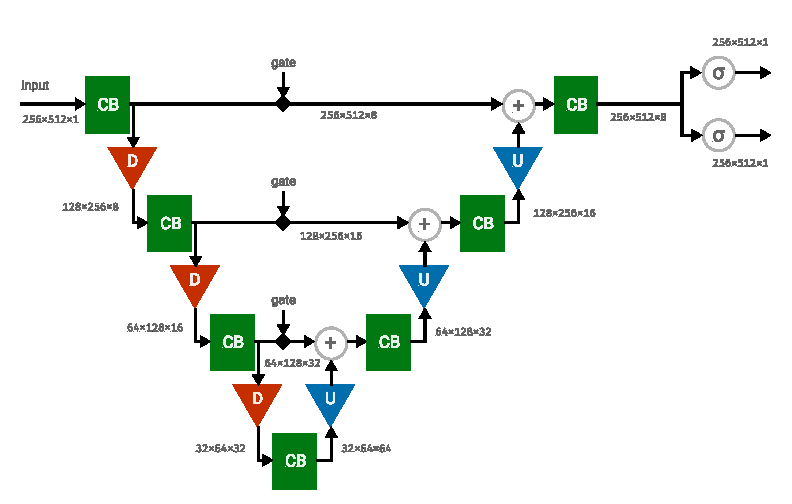
\includegraphics[width=140mm]{../img/architecture-complete.pdf}
    \caption{TODO}
    \label{fig:ArchitectureCombined}
\end{figure}

We choose to share the entire U-Net model for both the supervised and unsupervised tasks. The two tasks are differentiated only at the very last layer. The original U-Net architecture ends with a 1x1 convolution layer with sigmoid activation. It can be viewed as a pixelwise softmax for two output classes of a typical classification model. We decided to fork the architecture here, having one sigmoid convolution for the supervised segmentation task and one for the unsupervised reconstruction task.

The supervised task can be trained in almost the same way as the the original U-Net archtiecture:

\begin{itemize}
    \item A batch $(x, y)$ of input images and expected segmentation masks is taken from the dataset.
    \item Input images $x$ are fed through the model, producing a prediction for the segmentation mask $\hat{y}$ and for the reconstructed image $\hat{x}$.
    \item A loss function is used, computing the distance between $y$ and $\hat{y}$ and generating gradients for the network.
    \item Reconstruction output $\hat{x}$ is ignored and no gradients for the branch are computed.
    \item An optimizer uses computed gradients to update model parameters.
\end{itemize}

The unsupervised task could be trained in the same way, using the other output branch of the model. This would work for a typical autoencoder, but since the U-Net architecture contains skip connections, the model could learn an identity function without using any of the abstraction-learning layers. The goal of unsupervised learning is learning these abstract features, so this training scheme is infeasible in our context.

We propose two ways of overcoming this challenge:

\begin{itemize}
    \item gated skip connections
    \item denoising
\end{itemize}

One option is to disable skip connections during reconstruction training and keep them enabled during segmentation training. This should force the model to learn abstract features during reconstruction, while also being able to utilize skip connections during segmentation. This scheme performs much better than a typical autoencoder without any skip connections, but is still outperformed by the next proposed scheme (see detailed comparison in section \ref{sec:SkipConnections}).

The second option is to add some noise to the input image during reconstruction training. The model would learn to not only reconstruct the input image, but also to remove the added noise. We took inspiration from denoising autoencoders [CITE AUTOENCODERS]. The difficult part is designing the noise function such that it would cause the model to learn abstract representaions (see section \ref{sec:NoiseGeneration}).

We consider the described scheme for unsupervised U-Net training to be the main contribution of this thesis. The proposed experiments try to assess the viability of the scheme in the context of semi-supervised learning.

Both the segmentation and reconstruction tasks are trained jointly on composite batches and a single composite loss function. A single optimizer step is used to update model parameters for both tasks somultaneously. The process is described in detail in section \ref{sec:Training}.

The last sigmoid layers output images with only one channel. For the reconstruction output, this data is interpreted as a grayscale image. For the segmentation output, it represents the probability the model assigns to each pixel of being in the target class. This means that the model can learn to segment only one symbol class.

Hajič et al. [CITE] have explored the option of having multiple segmentation output channels. The hypothesis is that having the model learn multiple classes would improve its accuracy, since some internal representations can be shared. An added advantage is the reduced inference time as multiple segmentation masks can be infered in a single pass. Such a training however introduces problems related to unbalanced class distribution in the training data. Even if these can be overcome, their results suggest minimal accuracy benefits and a risk of decreasing accuracy in some cases.

Despite the fact that our experiment source code lets us easily train multiple classes, we choose not to explore this path as we are interested in the semi-supervised effects only.

\begin{figure}[p]
    \centering
    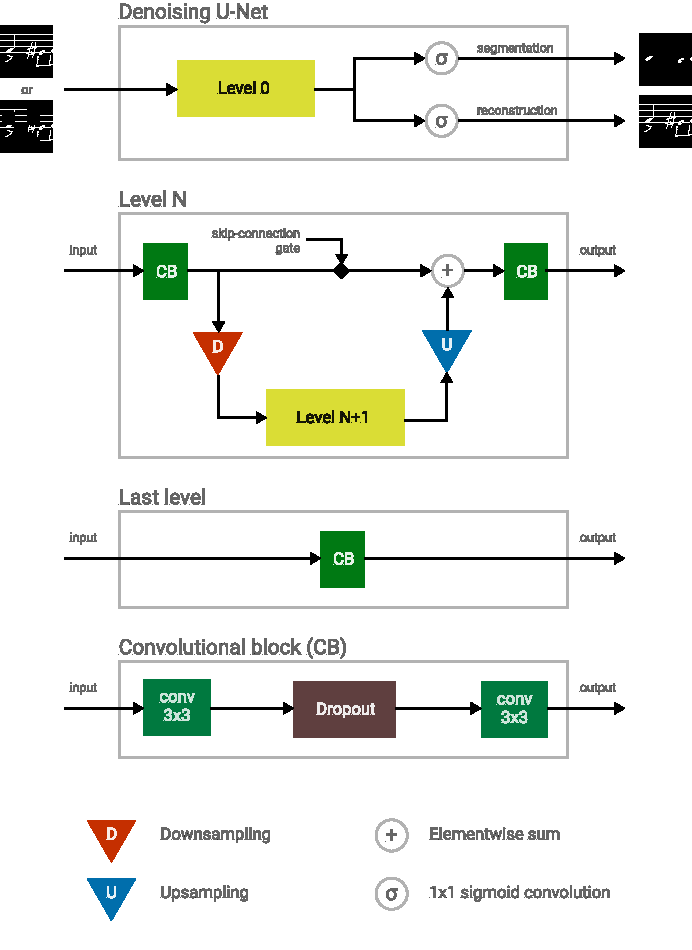
\includegraphics[width=140mm]{../img/architecture-pieces.pdf}
    \caption{TODO}
    \label{fig:ArchitecturePieces}
\end{figure}

The figure \ref{fig:ArchitecturePieces} contains a recursive block diagram of our extended U-Net architecture. The model takes a single image as the input and produces both the segmentation mask and the reconstructed image. When training segmentation, the reconstructed image is ignored and when training reconstruction, the input image is covered in noise and the output segmentation is ignored.

Each level of the network begins and ends with a convolutional block (CB). It consists of two identical 3x3 convolutional layers with an optional dropout layer in between them. Both convolutional blocks on the same level output the same number of feature channels. The number of feature channels is dictated by a hyperparameter we call \emph{inner features}. If the network has 4 inner features, the zero-th level convolutions output 4 feature channels. Each successive level then has twice as many feature channels as the one above it (e.g. 4, 8, 16, 32). The figure \ref{fig:ArchitectureCombined} contains image dimensions and channel counts for each edge in the network. The image dimensions are taken with respect to an input image tile of size 512x256.

The downsampling block is implemented as a 2D max pooling layer [CITE]. The number of feature channels is preserved. If we track the feature count through the encoder, we always first double the number of channels in the convolutional block and then reduce the spatial dimensionality in half in the downsampling block. This way the model can learn to extract higher-level features, before the spatial resolution is lowered. Since the image is two dimensional, halving the resolution shrinks the number of pixels to one quarter. Combined with the doubling of channel count, one encoder level effectively discards half of the image data. This acts as a bottleneck, forcing the network to learn relevant high-level representations.

The upsampling block has to perform two operations:

\begin{itemize}
    \item double the spatial dimensions
    \item halve the channel count
\end{itemize}

The resolution increase is performed by nearest neighbour interpolation (each pixel is copied to form a 2x2 region of the output image). The reduction in channel count is performed by a 1x1 convolutional layer, which can be trained to select or combine specific input channels. The upsampling output image may also be padded by zeros, if the desired output resolution is not even (we need to exactly match the resolution of the skip connection).

The gate on the skip connection is implemented as a multiplication by one or zero. This also causes any back-propagating gradients to be zeroed out, when the gate is closed. We took inspiration for the gating implementation from LSTM and GRU cells used in recurrent neural networks [CITE, CIRE].

The output of the upsampling block and the skip connection is merged in an elementwise sum operation. The original U-Net paper uses concatenation [CITE], however Dorfer et al. have shown that using a sum instead speeds up training, while having minimal impact on model accuracy [CITE].

In all layers (except for the two output sigmoid layers) the exponential linear unit (ELU) activation function is used. The reasons for this are described in section \ref{sec:ActivationFunction}.


\section{Datasets}
\label{sec:Datasets}

When performing experiments, we will use these three datasets:

\begin{itemize}
    \item CVC-MUSCIMA [CITE]
    \item MUSCIMA++ [CITE]
    \item DeepScores v2 [CITE]
\end{itemize}

These are the only datasets in the OMR field that contain semantic segmentation labels (for Common Western Music Notation). A comprehensive list of available OMR datasets is maintained by Alexander Pacha on his GitHub page\footnote{\url{https://apacha.github.io/OMR-Datasets/}}.


\subsection{CVC-MUSCIMA}

This dataset was introduced in the article \emph{CVC-MUSCIMA: A ground truth of handwritten music score images for writer identification and staff removal} [CITE]. It contains 1000 pages of handwritten music, created by having 50 writers transcribe 20 unique music pages. It was designed for the tasks of staff removal and writer identification. It is also the only handwritten music dataset, consisting of entire music pages -- all other handwritten datasets contain only individual symbols. This makes it very important for research focusing on symbol detection.

\begin{figure}[ht]
    \centering
    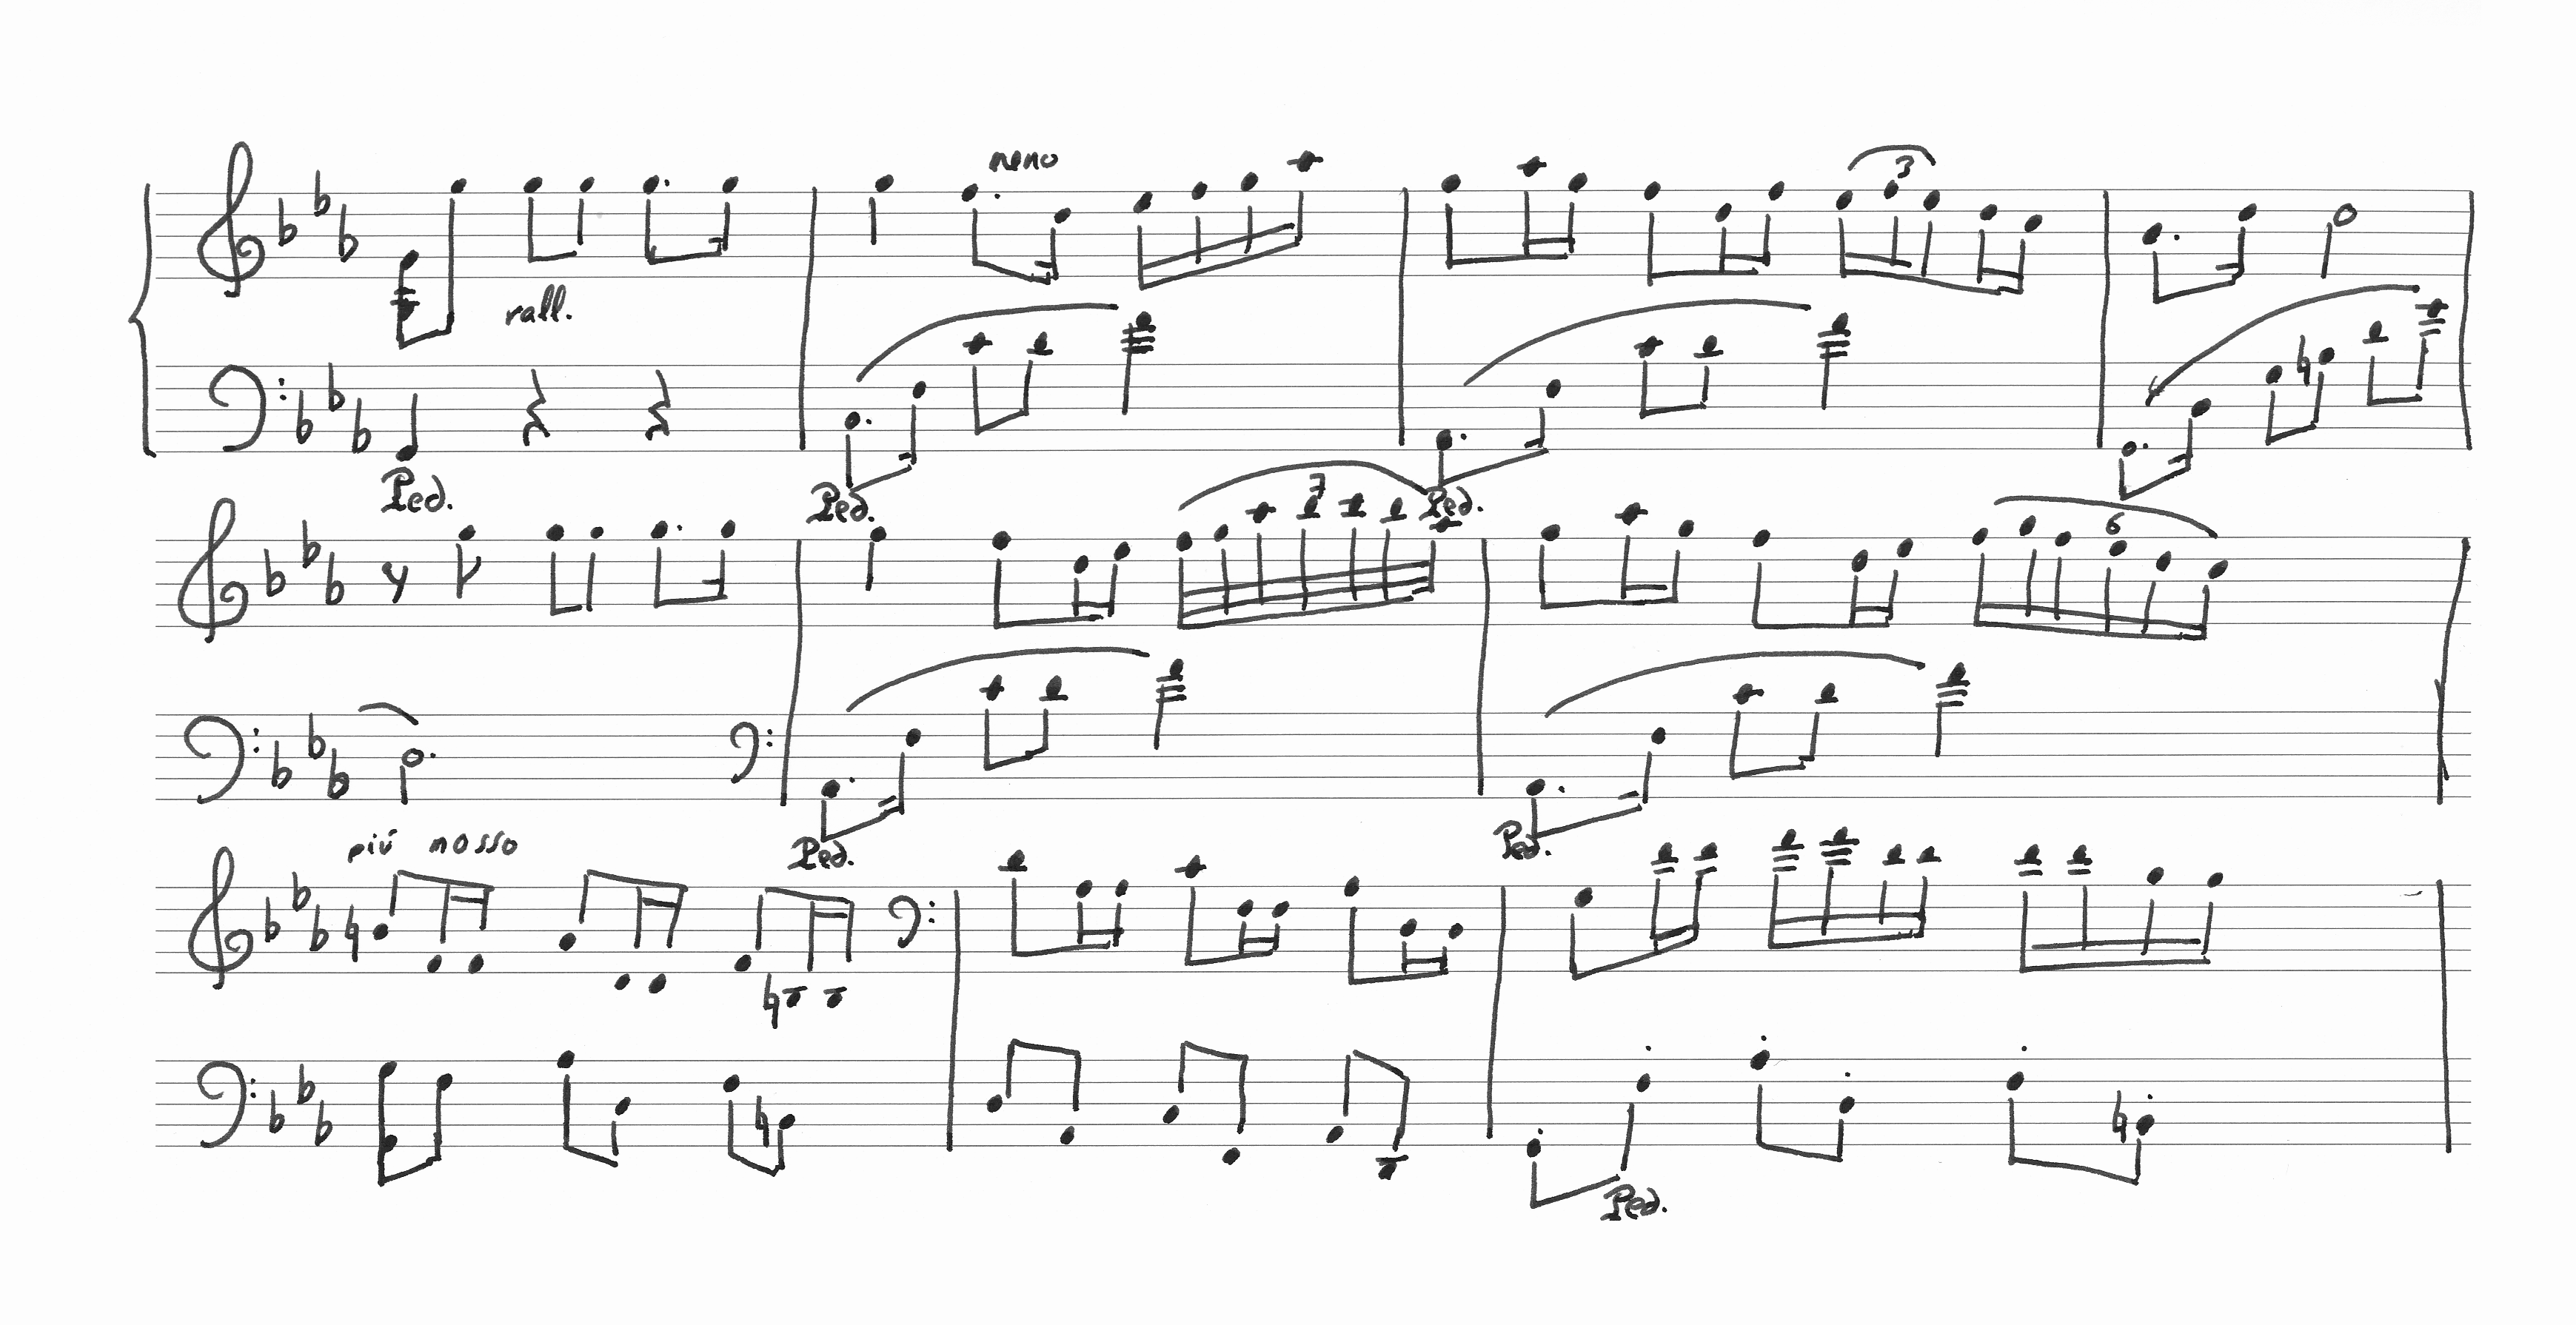
\includegraphics[width=140mm]{../img/cvc-muscima.png}
    \caption{One page from the CVC-MUSCIMA dataset. Image taken from the website \url{http://www.cvc.uab.es/cvcmuscima/index_database.html}}
    \label{fig:CvcMuscima}
\end{figure}

Since the dataset does not contain segmentation labels, we will use it primarily as a source of unlabeled training data.


\subsection{MUSCIMA++}

MUSCIMA++ was created by Jan Hajič jr. and Pavel Pecina as a general-purpouse OMR dataset. It was introduced in the article \emph{In Search of a Dataset for Handwritten Optical Music Recognition: Introducing MUSCIMA++} [CITE]. The dataset builds on top of the CVC-MUSCIMA dataset, providing rich annotations for 140 selected pages. The annotation scheme was designed to be sufficiently low-level for tasks such as object detection (bounding boxes, symbol classes, segmentation masks), while also having relationship data in the form of an oriented graph, that lets a user extract semantic information about the music. Dataset authors call this annotation scheme the \emph{Music Notation Graph} (MuNG).

\begin{figure}[ht]
    \centering
    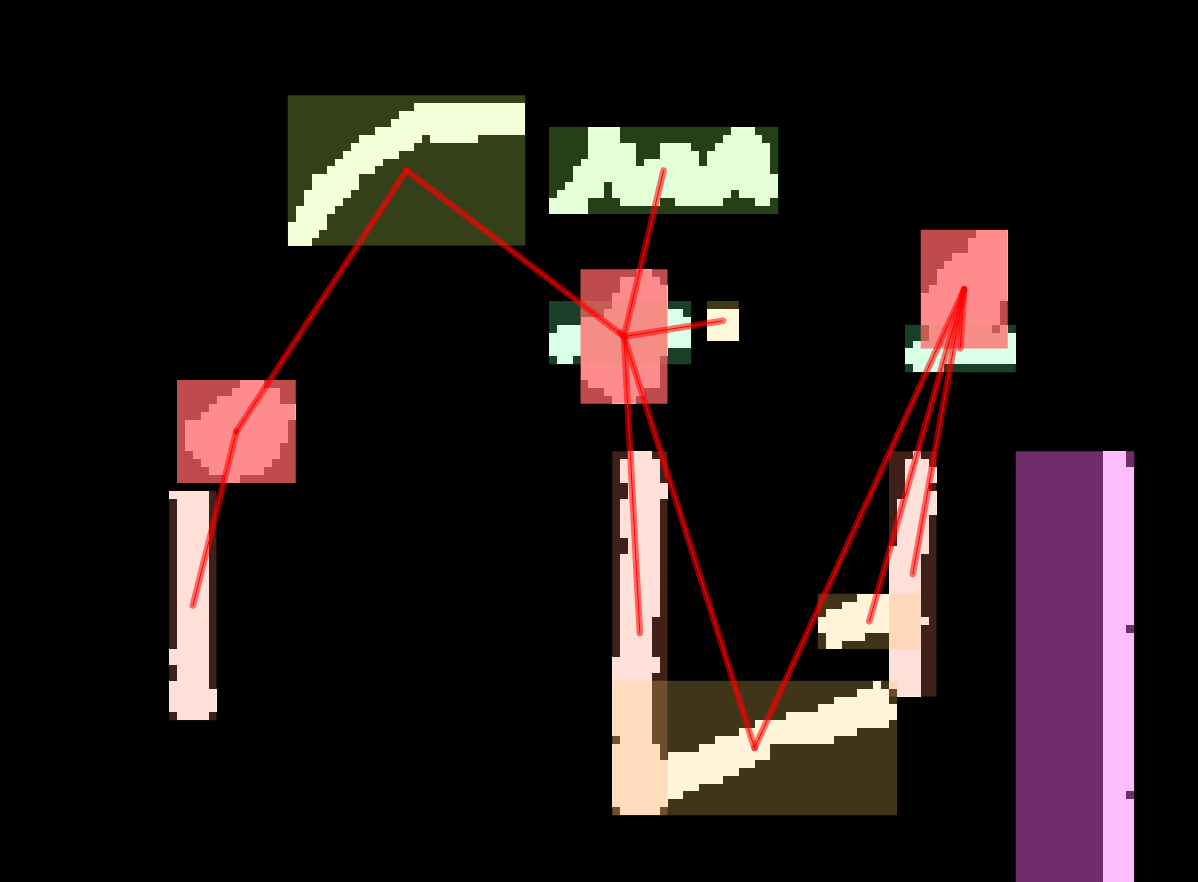
\includegraphics[width=100mm]{../img/muscima-pp.png}
    \caption{Annotations present in the MUSCIMA++ dataset (bounding boxes, segmentation masks and the notation graph). The image is taken from [CITE]}
    \label{fig:MuscimaPP}
\end{figure}

The dataset was updated in 2019, fixing bugs and modifying class names to be aligned with the SMuFL\footnote{\url{https://www.smufl.org/}} standard. A similar update was also performed on the DeepScores dataset [CITE], making it easier to use both datasets simultaneously. The latest dataset description and accompanying tools can be found on the GitHub page\footnote{\url{https://github.com/OMR-Research/muscima-pp}} of the OMR Research group\footnote{\url{https://omr-research.net/}}.

We will use this dataset as a source of labeled data for semantic segmentation.


\subsection{DeepScores}

The version 2 of this dataset was introduced in the article \emph{The DeepScoresV2 Dataset and Benchmark for Music Object Detection} [CITE]. The dataset contains entire pages of printed music, with annotations best suited for object detection, semantic segmentation and object classification. It was created from MusicXML documents taken from the MuseScore\footnote{\url{https://musescore.com/sheetmusic}} website and engraved using the LilyPond\footnote{\url{https://lilypond.org/}} tool. The dataset contains 255,386 pages of music, but also provides a dense and diverse subset, having only 1,714 pages. The version 2 also introduced a MUSCIMA++ compatibility mode, making it easier for the two datasets to be used simultaneously.

\begin{figure}[ht]
    \centering
    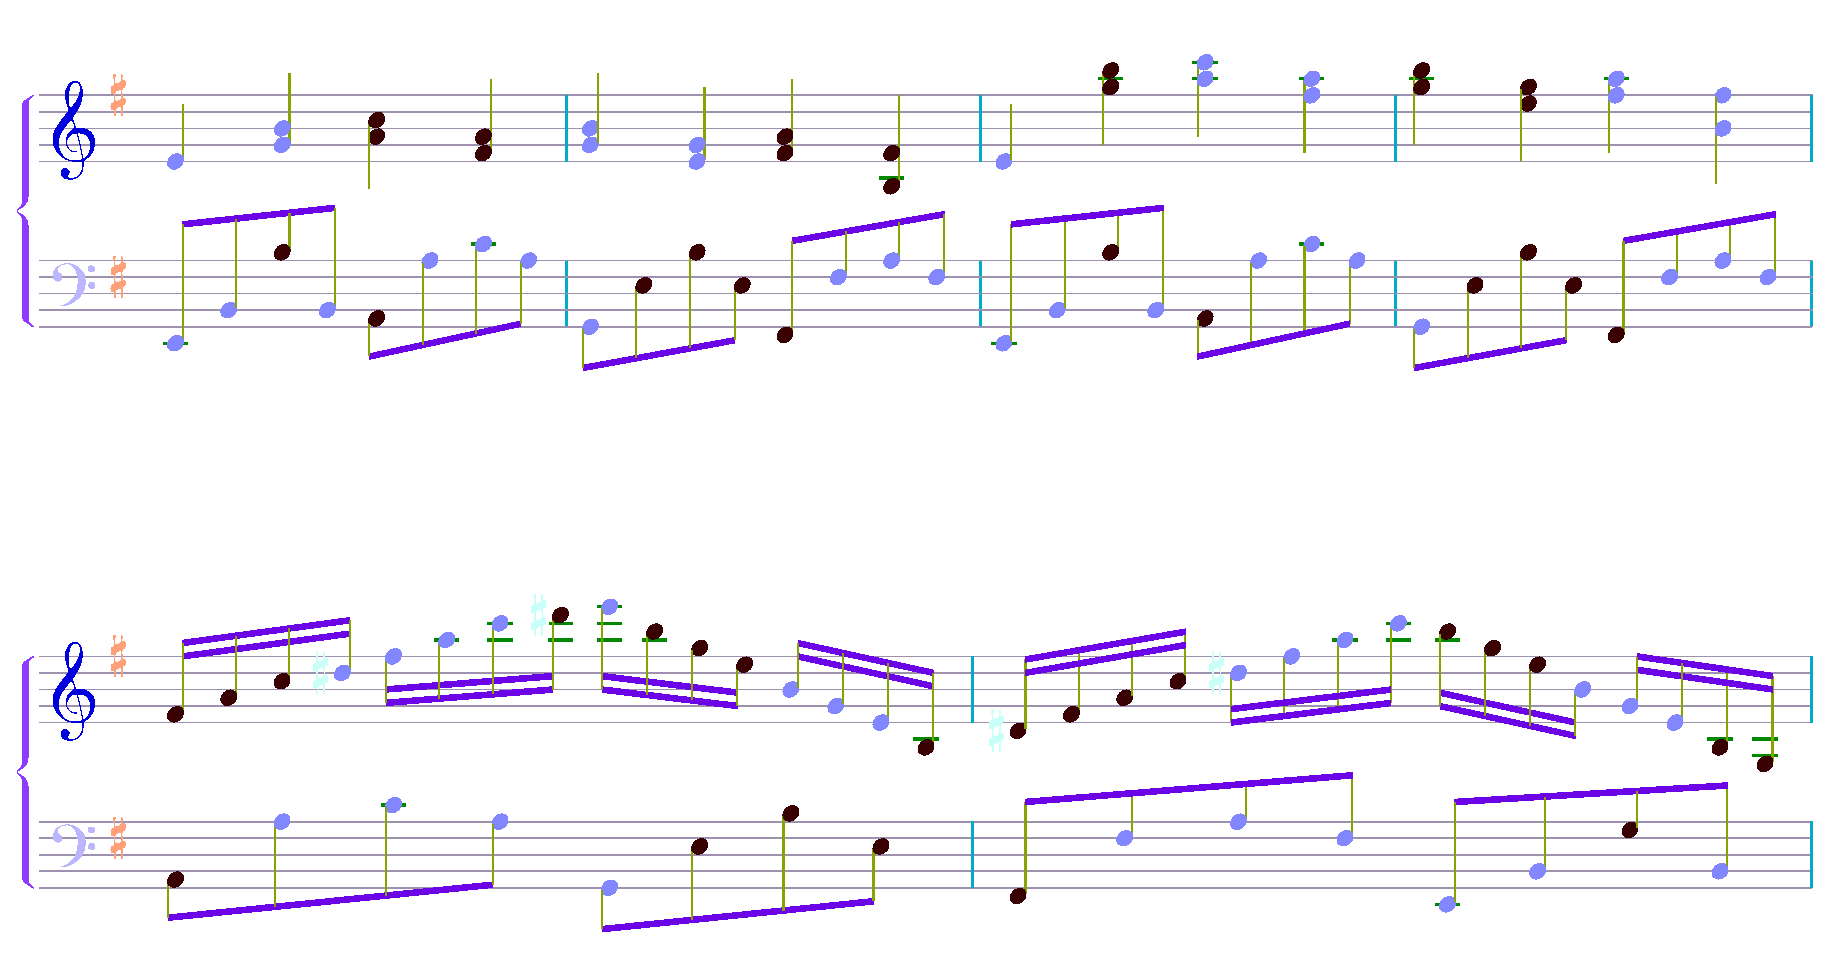
\includegraphics[width=140mm]{../img/deepscores.png}
    \caption{An example of the semantic segmentation labels from the DeepScores v2 dataset. The dataset is very large, but digitally engraved.}
    \label{fig:DeepScoresV2}
\end{figure}

We will use this dataset as a source of labeled data for semantic segmentation.


\subsection{Combining datasets}

We would like to slice and combine described datasets in various ways, depending on the performed experiment. There are two operations we want to perform:

\begin{itemize}
    \item Split an existing dataset into multiple slices (e.g. validation, supervised and unsupervised slices).
    \item Combine two different datasets together.
\end{itemize}

The splitting is needed for an experiment, that gradually increases the amount of unlabeled data and measures the change in model accuracy. This means the splitting logic has to be stable with respect to the size of the unlabeled slice:

\begin{itemize}
    \item We do not want the content of other slices to change, when we change the size of the unlabeled slice.
    \item We want the unlabeled slice to only gain new data, not to be completely resampled.
\end{itemize}

This stability is achieved by giving consideration to the splitting logic (sampling the unlabeled data as the very last slice) and to the shuffling logic (the data is shuffled prior to splitting). All the randomness in the process is controled by a parameter called \emph{dataset seed}, which is distinct from the plain \emph{seed} used for other initialization (model weights and noise generation). Introduction of the \emph{dataset seed} is essential for isolating our experiments from variability introduced by differential dataset sampling.

One additional consideration has to be made when sampling datasets CVC-MUSCIMA and MUSCIMA++. Since their content consists of music transcribed by 50 different wirters, we would like our splits to keep these writers separate. Anotherwords we do not want a single writer to be present in both the training set and the validation set. We enforce this constraint to better measure the ability of the trained model to generalize. The official test set of MUSCIMA++ built with this approach is called the \emph{writer-independent test set}, therefore we will call this property of our splitting logic \emph{writer-independence}.

% TODO: figure - splitting logic in an example "all" -> "shuffle" -> "splits"

When combining datsets, we run into the problem of image resolution. Since our proposed architecture learns visual features in scale-dependant way, we need to bring all datasets to the same resolution. Datasets CVC-MUSCIMA and MUSCIMA++ have the same source images, so the problem is not present here, however the dataset DeepScores is sampled at a lower resolution. In paper printing, a unit of DPI (dots per inch) is used. We cannot, however, use this unit, since it would assume the music from both datasets has the same size when printed on paper. A more general approach would be to define a unit, that could be derived from the raster image itself, without any knowledge of the scanning/printing DPI. The open format MusicXML\footnote{\url{https://www.musicxml.com/}} uses a spatial unit defined as \emph{one tenth of interline space} (the distance between two adjacent stafflines). We took inspiration form this and defined a unit we call DPSS (dots per staff space). DPSS of a raster music document is the number of pixels between two neighbouring stafflines. We measured the DPSS of CVC-MUSCIMA to be \verb`28.75 px` and of DeepScores to be \verb`16.0 px`.

% TODO: figure - visualization of DPSS in MUSCIMA++ sample

When matching the resolution of both datasets, we need to perform image resizing and we need to choose the target size and the interpolation method. We ended up upscaling the DeepScores dataset to match the resolution of the CVC-MUSCIMA dataset with the bilinear interpolation method.

In the beginning we tried downscaling CVC-MUSCIMA with area interpolation method. We chose the area method because it does not produce aliasing artifacts (it works by averaging pixel values over an area). It, however, introduced problems with thin lines (such as stafflines and stems) that faded below 50\% intensity on most pixels. That caused the pixelwise F1 score we use to evaluate the experiments to become very noisy and difficult to interpret.


\section{Noise Generation}
\label{sec:NoiseGeneration}

Typical denoising autoencoders are used either for removing noise from existing images (say, an overlayed text, sensor noise, or aliasing artifacts) or for learning abstract features [CITE]. If noise is sufficiently fine, as to not obstruct the high-level structure of the image, the autoencoder can learn this high-level structure in an unsupervised way. This setup can be used for feature extraction, similar to how variational autoencoders are used [CITE VAE].

Our goal is to leverage this training scheme to force our U-Net model to learn high-level representations. We chose to use noise in the form of dropping out parts of the input image -- setting the image pixels to zero. The parameter that specifies the percentage of zeroed-out image area is called \emph{noise dropout}.

We could decide for each pixel independently, whether it should be dropped, but that would produce a very fine noise. We belive that such a noise would not force the model to learn large symbols, as they are unnecessary for removing the noise. Therefore we chose to increase the resolution of the noise to form a square grid, where one square covers approximately two staff spaces. Such a noise drops out large enough sections, that simple operations like dilation will not fix it, while at the same time being small enough that the number of plausible reconstructions within the dropped space is reasonably limited. An extreme situation would be dropping the entire input image, but there the space of possible reconstructions would be so large, that it would be impossible for the model to guess the correct one (even among the space of plausible reconstructions).

% TODO: image, comparing various noise sizes

We got the idea of dropping image squares after reading the article by [CITE CUNEIFORMS]. The authors of the article present a method for reconstructing parts of an input image using a generative adversarial network. Their goal is to create synthetic training data for the task of cuneiform sign recognition.


\section{Training}
\label{sec:Training}

There are many options in how a semi-supervised generative model is trained. One option is to pre-train a model in the unsupervised mode and after that train a separate supervised part of the model [CITE KINGMA 2014]. Another option is to run the supervised training as a fine-tuning step after the unsupervised training, similar to the transfer learning approach [CITE TRANSFER LEARNING]. We chose to train both the supervised and the unsupervised tasks simultaneously, using a single, composite loss function.

One training step has the following structure:

\begin{itemize}
    \item An input image is passed through the network and the produced segmentation is compared to the gold one, producing the supervised loss.
    \item An input image with noise added is passed through the network and the produced reconstruction is compared to the clean input image, producing the reconstruction loss.
    \item The reconstruction loss is multiplied by a constant hyperparameter we call \emph{unsupervised loss weight}. Both losses are summed to produce the composite loss.
    \item The composite loss is used to calculate model gradients.
    \item An optimizer uses these gradients to update model weights.
\end{itemize}

The input to the training step is a composite batch of $(x_l, y_l)$ labeled data pairs and $(x_u, y_u)$ unlabeled data pairs.

\begin{itemize}
    \item $x_l$ are input images for segmentation
    \item $y_l$ are gold segmentation masks
    \item $x_u$ are noised input images for reconstruction
    \item $y_u$ are cleaned target reconstruction images
\end{itemize}

The number of labeled and unlabeled pairs in a composite batch differs and their ratio is related to the ratio of labeled to unlabeled data in the dataset. The hyperparameter \emph{batch size} dictates the total number of labeled and unlabeled pairs in one composite batch.

% TODO: image that illustrates the batching process (input data -> batched data)

Composite batches are created by taking training pairs from the labeled and unlabeled splits of the dataset. When the next pair is taken, we either take it from the labeled or the unlabeled split, whichever is larger, with respect to their target ratio. For example, if their ratio in the whole dataset is 1:5 (labeled to unlabeled) and we have 10:201 remaining pairs, we will take an unlabeled pair next. We take pairs until we have \emph{batch size} number of them and then we send them to the training logic as a new composite batch.

To be able to batch together the training images, they need to have the same spatial dimensions. For this reason we do not train on the entire music pages, but instead on tiles of fixed size. The size is set to 512 pixels wide and 256 pixels high for all experiments. We took inspiration for this from the article by [CITE Hajič]. The tiles are sampled from the music page at random locations and the number of tiles is equal to the area of the page, divided by the area of the tile. The article also employs a technique called oversampling, where a tile is sampled up to five times if it contains no pixel of the target segmentation class. This technique helps with training on rare symbols (e.g. clefs), where most tiles would contain no instance of the target class. Our training logic also implements this oversampling technique.

The semantic segmentation task is usually framed as a pixelwise classification problem. For this reason we use the pixelwise binary crossentropy loss function [CITE DL BOOK]. To make the loss value \emph{batch size} and \emph{tile size} invariant, we compute the average over all pixels in a batch. This allows us to sum the supervised and unsupervised losses, as they are of a similar magnitude, regardles of the number of labeled and unlabeled training pairs used. The reconstruction task will also use the same pixelwise binary crossentropy loss function, since the reconstruction of a single pixel can be understood as the probability of the pixel being black.

We use the Adam optimizer for all experiments, with learning rate $0.001$, $\beta_1 = 0.9$, $\beta_2 = 0.999$ and $\varepsilon = 10^{-7}$ [CITE ADAM]. Also for all experiments, we use the validation dataset to assess the performance of the model and train for as long as it is improving. Any evaluation of any trained model is performed by the model with the optimal validation dataset performance (unless the entire validation training curve is shown).


\section{Evaluation Metrics}
\label{sec:EvaluationMetrics}

Semantic segmentation is closely related to object detection and recognition. It is often performed as the first step from which object bounding boxes are computed. The segmentation output is first binarized by applying a threshold. Adjacent positive pixels are merged to form connected components, where each can then be enclosed in a bounding box. The described process is very basic and there are ways to improve it. A sligtly more advanced process in the context of notehead recognition is used in the article by [CITE DORFER].

There are many metrics that evaluate the correctness of predicted bounding boxes, comparing them to ground-truth bounding boxes. A metric called intersection over union (IOU) can be used to calculate the overlap of two bounding boxes. Setting a threshold on IOU and computing it between all pairs of predicted and ground-truth bounding boxes lets us compute the binary classification confusion matrix. From this matrix, additional metrics could be computed, such as precision, recall, and F1 score. By introducing a confidence level for each bounding box, or considering the performance over multiple classes, we get a large number of metrics that can be used to assess various aspects of the recognition. An article by [CITE PADILLA] provides an extensive comparison of all these metrics.

Even though these object detection metrics are more telling about the actual usefulness of the model (we care about detected objects, not pixels), we chose to evaluate our experiments directly at the pixel level. Adding these evaluation metrics adds unecesasry complexity to our experiments and it is not needed for our goal -- measuring the impact of unsupervised data.

We chose to use the pixelwise F1 score at 0.5 thresholding. The F1 score is computed as the harmonic mean of precision and recall, so that it is high, when both precision and recall are high. It is computed using the following formula from the confusion matrix:

$$
    F1 = \frac{2 \cdot TP}{2 \cdot TP + FP + FN}
$$

The confusion matrix values are computed over all pixels of the the entire (validation) dataset.

It is important to note, that the two articles regarding music symbol detection ([CITE hajič, dorfer]) use object detection F1 score, which is not directly comparable to our pixelwise F1 score.


\section{Semi-supervised Improvements}
\label{sec:SemisupervisedImprovements}

The main hypothesis this work is attempting to validate is that adding unlabeled data to the training process helps. We primarily want to improve model accuracy, but as we will see, this is not what our experiments suggest. They do, however, show improvements in other areas, such as training stability and reduced overfitting (section \ref{sec:UtilizingCvcMuscima}).

In the first experiment, we test how various labeled to unlabeled data ratios affect the training process. The experiment uses the MUSCIMA++ dataset [CITE]:

\begin{itemize}
    \item 10 pages act as the labeled set.
    \item 0, 5, 10 and 50 pages act as the unlabeled set.
    \item 10 pages act as the validation set.
    \item All of these pages come from the writer-independent train set of MUSCIMA++ and are chosen in a writer-independent manner (all the splits contain pages by different writers).
\end{itemize}

The learned task is notehead segmentation (both full and empty noteheads). Noteheads are an ideal symbol for this kind of measurement. Firstly, they are very abundant. Each page of the dataset contains many instances of them and they are evenly scattered over the whole page. If we were to instead detect more rare symbols (such as clefs or rests), it could skew the results, making it difficult to separate the effects we want to measure. Handwritten noteheads are also very diverse in style, making them more interesting to learn (compared to, say, stafflines).

All model hyperparameters are set to sensible deafults. The derivation of these values is desribed later in section \ref{sec:UnderstandingHyperparameters}. The model capacity, described by the \emph{inner features} parameter is set to 8, which is useful to know for comparison with the next experiment. The proposed dataset is rather small and so the training is very noisy (figure \ref{fig:ExplorationNoteheadsNoDropout}). To stabilize the trainig we set the dropout parameter to 50\% [CITE DROPOUT].

\begin{figure}[ht]
    \centering
    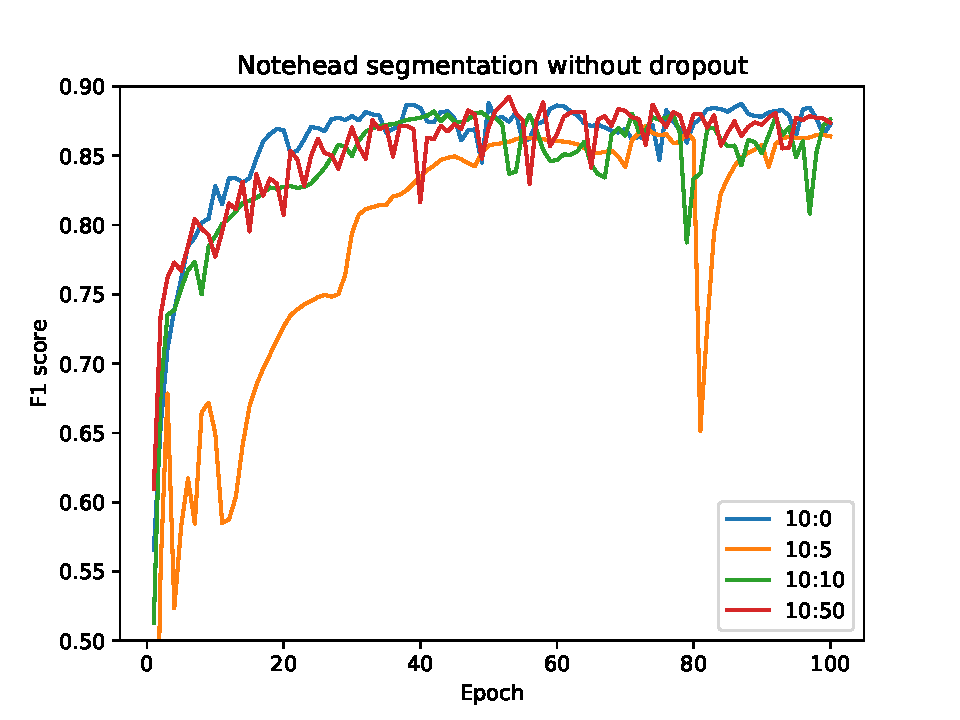
\includegraphics[width=140mm]{../../figures/01-exploration-noteheads/noteheads.pdf}
    \caption{Training on a small dataset without dropout is noisy, see the orange line at the beginning and the green line at the end.}
    \label{fig:ExplorationNoteheadsNoDropout}
\end{figure}

We expect that as we add more and more unlabeled data, the F1 score should reach higher and higher. Or at least not get worse. This is not what we see in the figure \ref{fig:ExplorationNoteheads}. The fully supervised model outperforms all the others by a clear margin.

Focusing only on the semi-supervised models, it seems that adding more unsupervised data maybe helps here, although the three lines end up on top of each other at the epoch 200. A better idea is to look at the figure \ref{fig:ExplorationNoteheadsEvaluation}. The chart contains evaluation results on the test set of six runs of each configuration. We can clearly see how the performance rises with more unsupervised data. Unfortunately it does not reach above the fully-supervised results. We unfortunately cannot push the amount of unlabeled data much higher, as it would break our training process (see section \ref{sec:BatchSize}) and it would likely also have diminishing returns. The actual numbers are summarized in table \ref{tab:ExplorationNoteheads}.

The reason for the drop in performance is actually caused by the fact, that the supervised model has to only learn one task -- segmentation. Whereas the semi-supervised one has to also learn the unsupervised reconstruction task. This claim is explored in the next section and is supported by the fact that the performance drop disappears when we increase model capacity.

\begin{figure}[p]
    \centering
    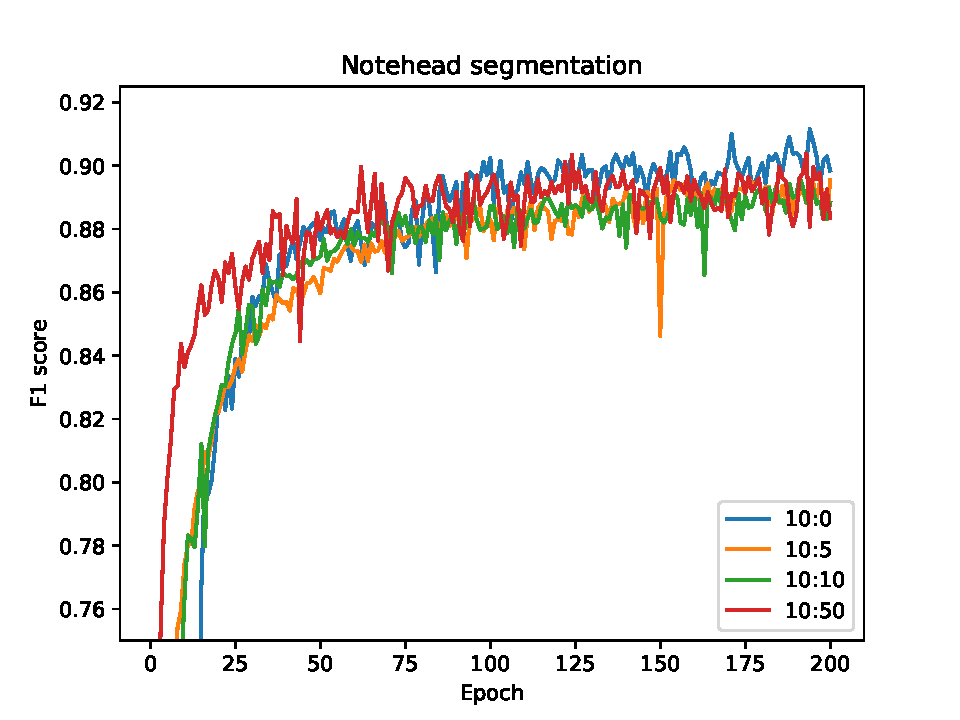
\includegraphics[width=140mm]{../../figures/01-exploration-noteheads/noteheads-dropout.pdf}
    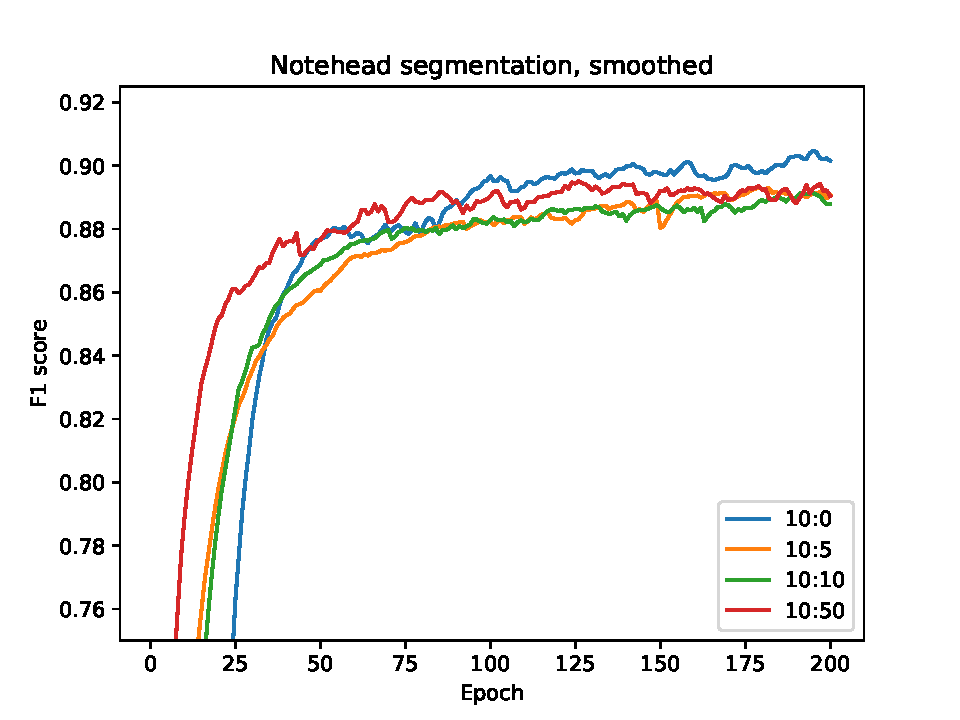
\includegraphics[width=140mm]{../../figures/01-exploration-noteheads/noteheads-dropout-smooth.pdf}
    \caption{Lorem ipsum dolor.}
    \label{fig:ExplorationNoteheads}
\end{figure}

\begin{figure}[ht]
    \centering
    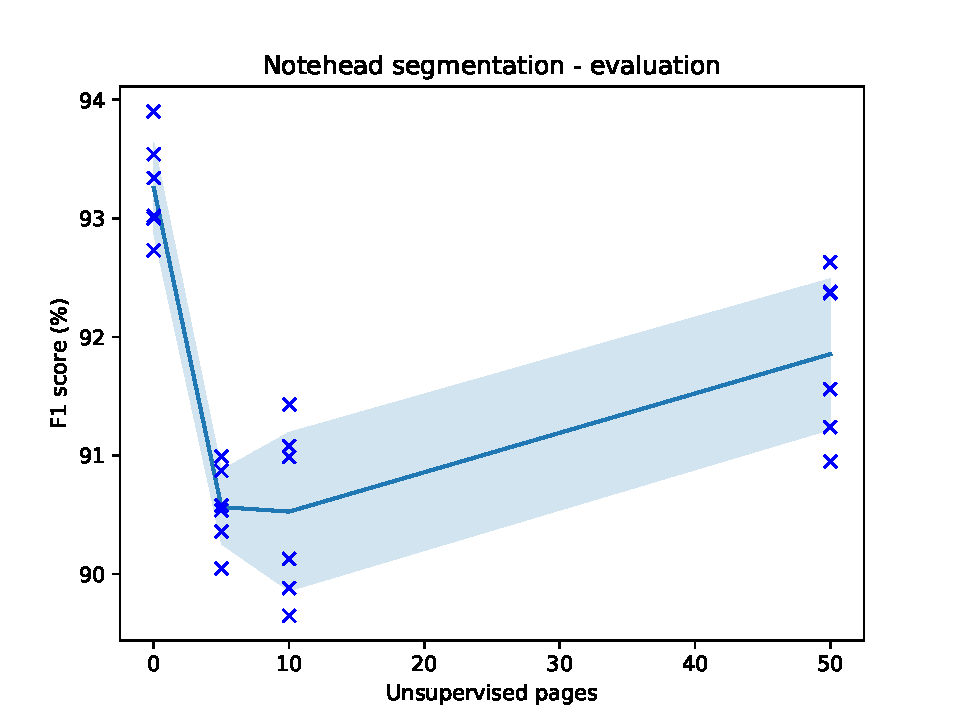
\includegraphics[width=140mm]{../../figures/01-exploration-noteheads/noteheads-evaluation.pdf}
    \caption{Lorem ipsum dolor.}
    \label{fig:ExplorationNoteheadsEvaluation}
\end{figure}

\begin{table}[b!]
    \centering
    \begin{tabular}{l@{\hspace{1.5cm}}D{.}{,}{3.2}D{.}{,}{1.2}D{.}{,}{2.3}}
        \toprule
        & \mc{} & \mc{\textbf{Směrod.}} & \mc{} \\
        \pulrad{\textbf{Efekt}} & \mc{\pulrad{\textbf{Odhad}}} & \mc{\textbf{chyba}$^a$} &
        \mc{\pulrad{\textbf{P-hodnota}}} \\
        \midrule
        Abs. člen     & -10.01 & 1.01 & \mc{---} \\
        Pohlaví (muž) & 9.89   & 5.98 & 0.098 \\
        Výška (cm)    & 0.78   & 0.12 & <0.001 \\
        \bottomrule
    \end{tabular}
    \caption{Lorem ipsum dolor.}
    \label{tab:ExplorationNoteheads}
\end{table}

TODO: show visualization images / qualitative comparison between runs?


\section{Utilizing CVC-MUSCIMA}
\label{sec:UtilizingCvcMuscima}

This experiment attempts to address issues of the previous experiment:

\begin{itemize}
    \item fixed model capacity
    \item small dataset
\end{itemize}

In the chapter \ref{chap:CurrentStateOfOMR} we described the two major datasets for handwritten music recognition: CVC-MUSCIMA [CITE] and MUSCIMA++ [CITE]. The dataset MUSCIMA++ is a highly annotated subset of CVC-MUSCIMA. We can view both datasets together as a single semi-supervised dataset, being 12\% labeled and 88\% unlabeled. To the best of our knowledge, nobody has yet tried to utilize both datasets simulatenously for semantic segmentation.

Hajič jr. and Dorfer [CITE 1, 2] have used the U-Net architecture [CITE] for segmentation and they trained it on the MUSCIMA++ dataset. Their results are very impressive. Being able to further build on their work and improving the model by utilizing unlabeled data from CVC-MUSCIMA would be very helpful for the field of OMR. This experiment attempts to do just that.

We take the whole CVC-MUSCIMA dataset, separate writers from the MUSCIMA++ independent test set, separate 20 pages for validation set and remove other pages from these validation writers. The pages that remain are produced by writers not present in both the test set and the validation set. These remaining pages are partially contained in the MUSCIMA++ dataset (99 pages) and all the other pages are used as unlabeled data (551 pages). Therefore we train on 650 out of 1000 pages of the CVC-MUSCIMA dataset.

Since the dataset is now much larger than in the previous experiment (section \ref{sec:SemisupervisedImprovements}), we no longer need the dropout. In fact, the training is even more stable and individual runs are clearly separated.

This experiment attempts to compare fully-supervised and semi-supervised models, regardless of their capacity. We therefore train various model capacities (the \emph{inner features} model parameter) and then compare the best ones for each setting.

Another difference to the previous experiment is that the ratio of labeled to unlabeled data is fixed and given by dataset sizes. The ratio of 99 to 551 pages corresponds best with the ratio 10:50.

\begin{figure}[p]
    \centering
    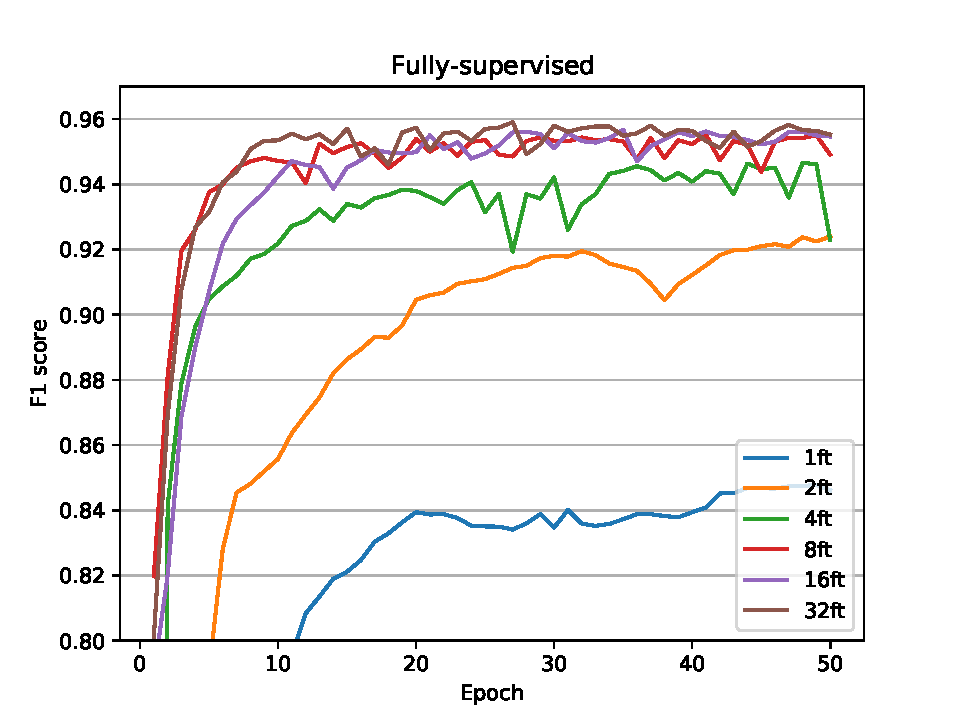
\includegraphics[width=140mm]{../../figures/02-cvc-improvements/supervised.pdf}
    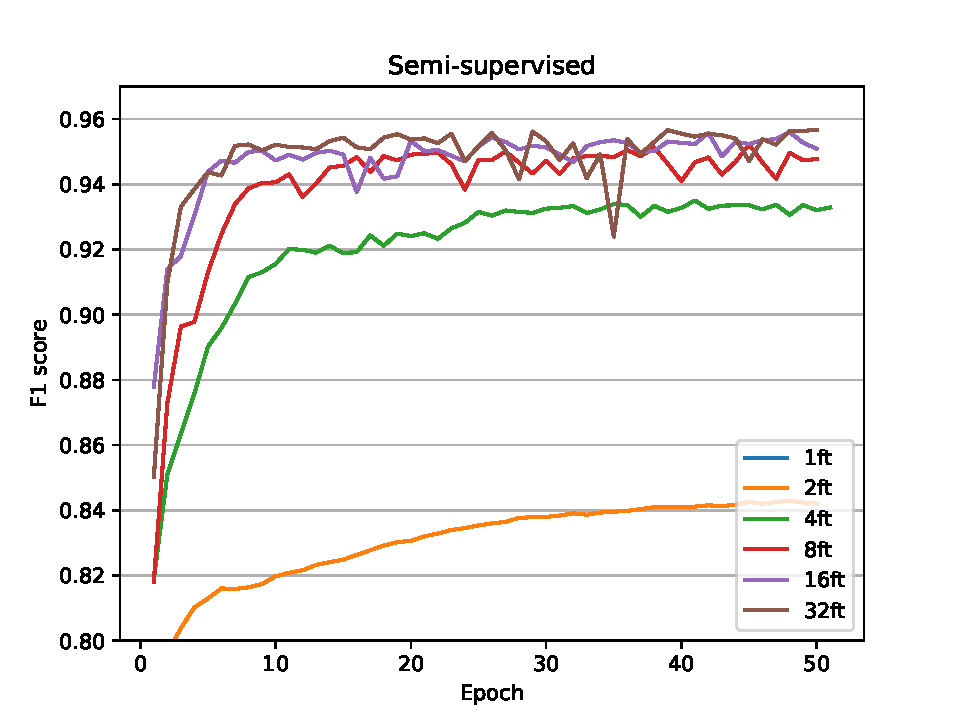
\includegraphics[width=140mm]{../../figures/02-cvc-improvements/semisupervised.pdf}
    \caption{Lorem ipsum dolor. TODO: the two improvements charts}
    \label{fig:CvcImprovements}
\end{figure}

The validation dataset F1 score over the course of training can be seen in figure \ref{fig:CvcImprovements}. In these charts we can see:

\begin{itemize}
    \item Models with 1 and 2 \emph{inner features} are clearly underfitting in the supervised mode (compared to other models). When we add the unlabeled data, their perfomance drops significantly, but the training curve gets much smoother.
    \item Models with 4 and 8 \emph{inner features} worsen much less and also get smoother (especially 4 becomes much more stable).
    \item Model 16 no longer worsens, it is able to learn both tasks.
\end{itemize}

Conclusions can be drawn from these observations:

\begin{itemize}
    \item The reconstruction and segmentation tasks clearly compete for model capacity. The performance drop of adding unlabeled data decreases, as the model capacity increases.
    \item The addition of unlabeled data can be used as a regularization technique. This is evident from the fact that training curves get much smoother as we add unlabeled data. A~regularization effect is also described in the corresponding literature [CITE SSL overview].
    \item All models come close to the 96\% line, but never cross it. While the semi-supervised models get as good as the fully-supervised, they never get better. It seems the reconstruction task is not learning any useful representations. [TODO: expand on this further and show reconstruction visualizations - they learn simple shapes, not abstract objects]
\end{itemize}


\section{Knowledge Transfer}
\label{sec:KnowledgeTransfer}

TODO: knowledge transfer experiment

\begin{figure}[ht]
    \centering
    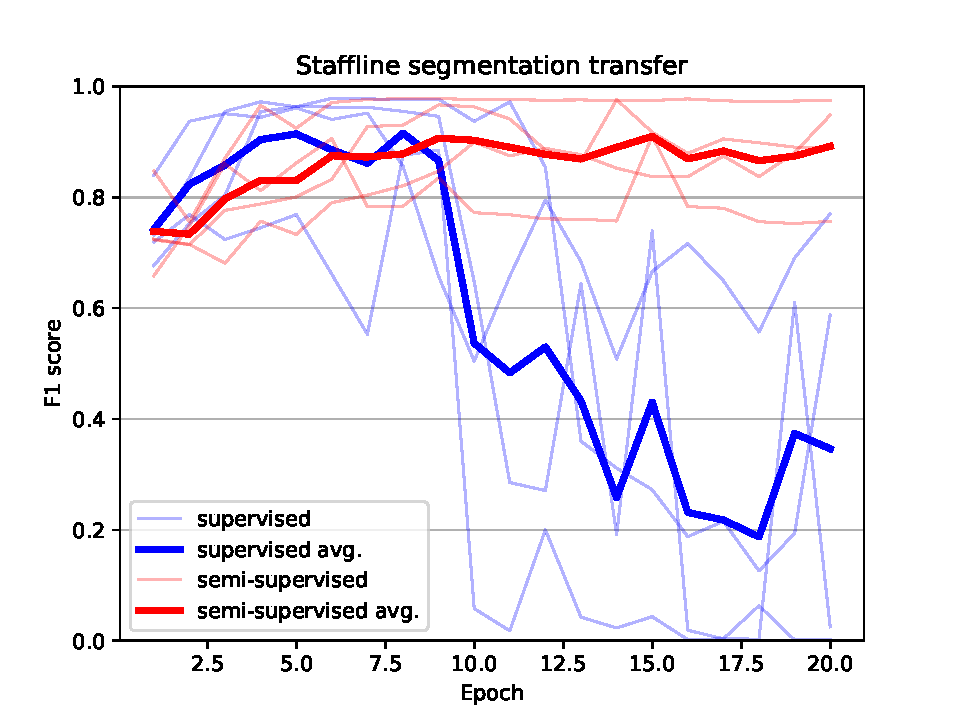
\includegraphics[width=140mm]{../../figures/04-staffline-transfer/transfer.pdf}
    \caption{TODO lorem ipsum}
    \label{fig:StafflineTransfer}
\end{figure}


\section{Understanding Hyperparameters}
\label{sec:UnderstandingHyperparameters}


\subsection{Batch Size}
\label{sec:BatchSize}

In the deep learning field, it is known that having a small batch size makes the training fast and noisy, whereas a large batch size makes it more stable at the cost of being slower [CITE DL BOOK]. Since our model is fully cconvolutional and we train it on image tiles of fixed size, we can consider the size of these tiles to be a parameter similar to batch size. It also regulates the amount of data used for gradient estimation. If the tiles are large enough, we can get away with batch size of 1 (this is what the original U-Net article does [CITE]).

Using such a small batch size is, however, not possible in our case. Our training process expects batches containing both labeled and unlabeled data. Batch size determines the total number of these two kinds of data items in the single composite batch. The ratio of these two item types within the composite batch is dictated by the ratio within the whole dataset. So if our dataset has, for example, 1:5 labeled to unlabeled data, the batch size has to be at least 6. Otherwise we will start getting batches that contain only unlabeled data. This rule isn't as strict, since the model would probably learn both tasks even if half of all batches were missing labeled data, however if the imbalance becomes too severe, the training fails.

TODO: figure with the failing training (bs=2,ratio=1:10)

An example of such a failing training can be seen in figure TODO???. The model learns to perform reconstruction even for the segmentation task. This is understandable, since the two tasks are differentiated only at the last layer (1x1 sigmoid convolution). If all second-to-last layer activations contain image reconstruction data, then any 1x1 convolution combination of them will do as well.

Since all of our experiments have training data ratios between 1:0 and 1:10, we chose to set the batch size parameter to 10.


\subsection{Dropout}
\label{sec:Dropout}

We introduced dropout [CITE] when training on small datasets (section \ref{sec:SemisupervisedImprovements}). The training was so noisy, that it was difficult to infer any measurable differences between runs. Therefore we used dropout as a mean to stabilize the training. The model performace also sligtly increased in this setting.

When we train on larger datasets, the training is no longer unstable and dropout is not needed (section \ref{sec:UtilizingCvcMuscima}). In fact, it causes the training process to converge much slower (2x or more) and it does not perform any better.

Both the original U-Net article [CITE] and the article by Hajič jr. et al. [CITE] use the U-Net architecture without any dropout. In fact, an article by Thompson et al. [CITE] argues, that using traditional dropout on convolutional layers may not be ideal. This agrees with our findings, that dropout helps only in very specific circumstances.

It may be the case, that using batch normalization instead or dropout (like Hajič jr. et al. [CITE]) has the same effect of regularizing the network. However our goal is not to find the optimal architecture, but to measure the impact of unsupervised data. For that reason we did not explore this option.

From all this we conclude that dropout should be disabled by default.


\subsection{Skip Connections}
\label{sec:SkipConnections}

In the chapter about our architecture (\ref{sec:Architecture}) we described a method for disabling skip connections during reconstruction training. We have devised three modes for skip connection operation:

\begin{itemize}
    \item solid -- skip connections are always enabled, like in a typical U-Net archtiecture
    \item gated -- skip connections are enabled for supervised task (traitraining and inference) and disabled for reconstruction task (training and inference)
    \item none -- skip connections are always disabled, like in a typical autoencoder
\end{itemize}

The motivation behind gating skip connections is to compare the U-Net architecture (\cite{UNet}) to a more traditional fully-convolutional autoencoder archtiecture (\cite{AutoencodersOverview}).

We take the 16 \emph{inner feature}, semi-supervised model from experiment \ref{sec:UtilizingCvcMuscima} and train it with various skip connection settings. The training curves are shown in figure \ref{fig:SkipConnections}.

\begin{figure}[ht]
    \centering
    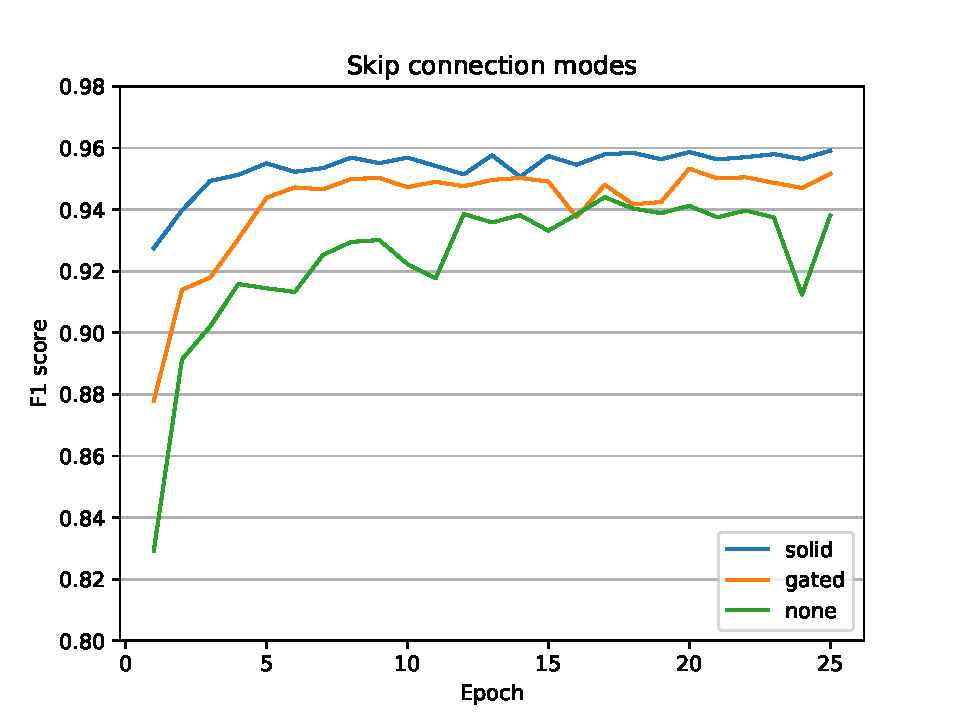
\includegraphics[width=140mm]{../../figures/05-skip-connections/skip.pdf}
    \caption{Comparing various skip connection modes with a model from experiment \ref{sec:UtilizingCvcMuscima} (16 inner features, semi-supervised). The permanent skip connection mode performs the best, although all runs are below the supervised baseline. The order could be different, should the baseline be exceeded.}
    \label{fig:SkipConnections}
\end{figure}

We can see that solid and gated modes have the best performance. The model with no skip connections is clearly worse at the segmentation task. This result validates the superiority of the U-Net architecture for semantic segmentation.

The gated mode seems to perform worse than the solid one. Despite this, we chose to train all the experiments in this gated mode as we belive it helps the model to learn representations during unsupervised training.

We have to point out, that all of our semi-supervised experiments never exceeded their supervised baselines. This means that bringing the model closer to its supervised setting (using solid skip connections) should increase its performance, because we are bringing it closer to the baseline. For this reason we cannot conclude, what the best skip connection mode would be, if we managed to exceed the baseline. It is possible the order of modes would get reversed. This is another reason why we chose to use gated connections, despite not being optimal in this experiment.


\subsection{Unsupervised Loss Weight}
\label{sec:UnsupervisedLossWeight}

This parameter determines the relative magnitude of the segmentation and the reconstruction loss. We first though this parameter would have significant impact in the training and would need to be tuned carefully. It turned out not to be the case. We ended up setting it 1 and not optimizing it.

Varying this parameter from 10 to 0.1 has minimal impact on model performance. When we examined the segmentation masks and reconstruction images as they evolve throughout the training process, we discovered that the primary impact is the change of speed of learning each task. When the parameter is 10, the reconstruction task is learned quickly and segmentation task is learned slowly. When we set it 0.1 the situation is reversed. If we let the training covnerge, it ends up learning both tasks equally well.

Interesting behaviour happens only at the extreme. When the parameter is set to zero, the reconstruction task produces no gradients and the training collapses to the fully-supervised regime. We performed an experiment that verified this behaviour.


\subsection{Noise Parameters}
\label{sec:NoiseParameters}

\begin{figure}[p]
    \centering
    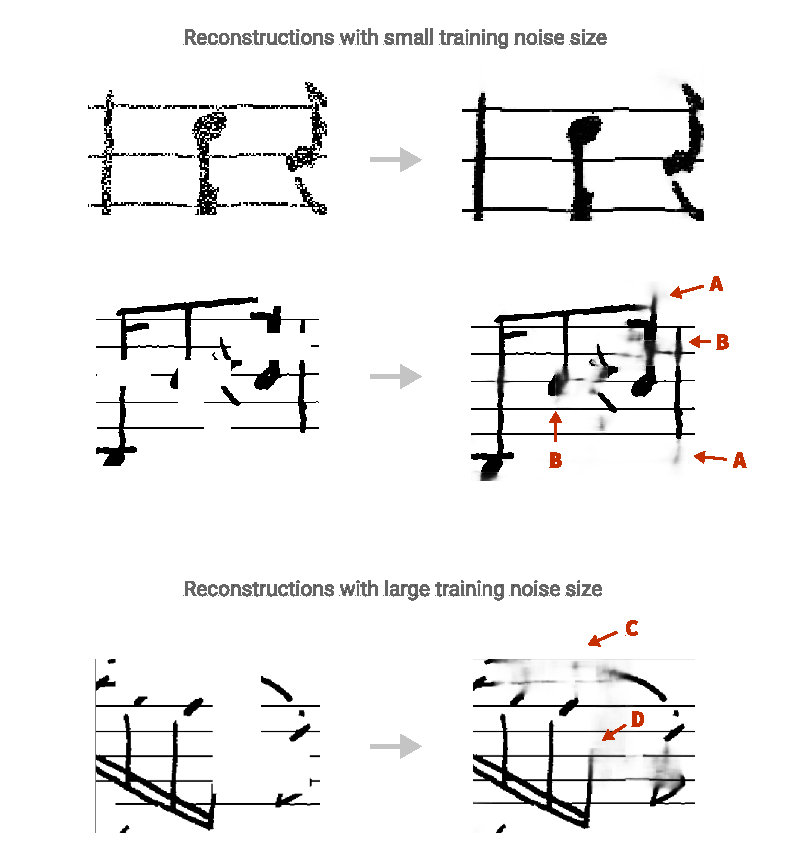
\includegraphics[width=140mm]{../../figures/06-noise/noise-size.pdf}
    \caption{Comparing reconstructions performed by models trained with small and large noise tiles. (A) Low-level reconstructions, make no sense in the musical context. (B) Visible edges of the dropped tiles in the reconstruction. (C) High-level reconstruction with staffliens and stems visible. (D) Forgotten notehead.}
    \label{fig:NoiseSize}
\end{figure}

There are two major nosie parameters that can be varied:

\begin{itemize}
    \item Noise resolution (size of dropout squares)
    \item Noise dropout ratio (ratio of erased input pixels)
\end{itemize}

In the section on noise generation (\ref{sec:NoiseGeneration}) we gave reasons for using larger noise resolution. We belive large tiles force the model to learn larger sybmols and thus the corresponding high-level representations. This hypothesis is supported by images shown in the figure \ref{fig:NoiseSize}.

The first two images show, how the model can learn to remove small noise easily. The model, however, does not produce satisfying reconstructions when applied to an image with larger noise tiles dropped, as seen in the second pair of images. We can see edges of the noise tiles still visible in the reconstruction, reconstructed stafflines fade when close to other symbols and most reconstructions are based on relatively low-level features. The beam corner is extended upwards, which is reasonable in the sense of drawing straight lines, but not in any musical sense. Comparatively, the lower two images show a much better reconstruction. The lower reconstruction was trained with noise size equal to the size seen in the lower left image. Reconstructed stafflines are sharp even when intersecting the eighth note and there are no tile edges visible (reconstructions blend well with the known image). The model has even managed to conjure up a fake set of stafflines and stems, that connect well to visible noteheads (pointer C). This shows that the model learns much higher-level features than just simple geometric shapes (lines, circles).

We ended up training all experiments with noise tiles of size equal to two staff spaces and noise dropout ratio of 25\%. We experimented with noise dropout of 50\%, but the performance seemed not to change. This chosen size and ratio can be seen in the last row of figure \ref{fig:NoiseSize}.


\subsection{Activation Function}
\label{sec:ActivationFunction}

We first used ReLU activation function (rectified linear unit) [CITE] in all convolutional layers (except the final sigmoid layer), just like it is used in the original U-Net article [CITE]. However, we occasionally encountered problems with convergence. Replacing the activation function with ELU (exponential linear unit) [CITE] solved these issues. We took inspiration from Hajič jr. et al. [CITE], who also use the ELU activation function. The difference between the two can be seen in figure \ref{fig:ActivationFunctions}.

\begin{figure}[ht]
    \centering
    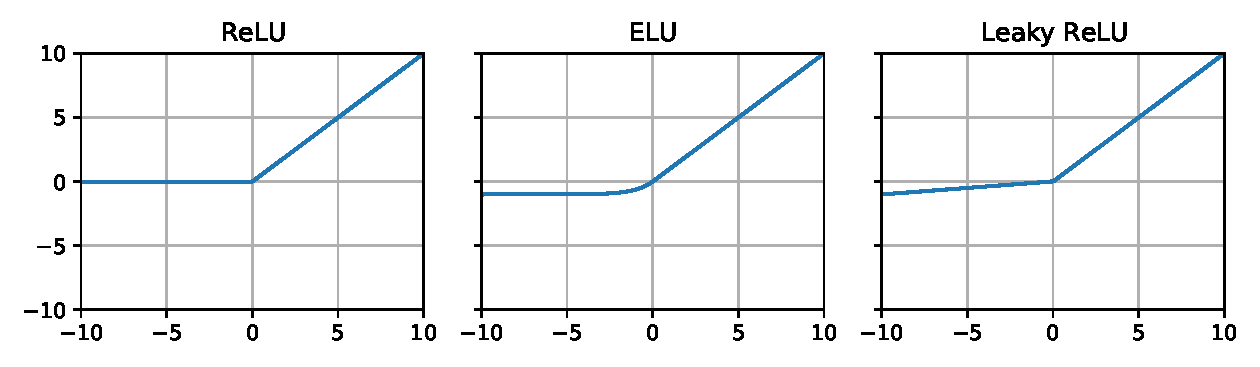
\includegraphics[width=140mm]{../../figures/03-activation-function/functions.pdf}
    \caption{Visualization of the explored activation functions. ReLU is flat in negative values and therefore has no gradient there. ELU has exponentially decaying gradient and leaky ReLU has a constant gradient. The parameter for the displayed leaky ReLU is 0.1 to make its shape more apparent.}
    \label{fig:ActivationFunctions}
\end{figure}

The convergence problems were happening at the very beginning of training. The model quickly learned to output a completely black image and never recovered from that state. We think it was an instance of the "dying ReLU" problem [CITE]. When the model is first initialized, it outputs a gray-ish image, since model weights are drawn from a uniform distribution centered on zero and the final sigmoid layer turns that into a 0.5 gray. Because the target images have black background, the model first learns to produce mostly black images. Only then does it learn to output white pixels as well (see figure \ref{fig:ActivationTrainingProgression}). With ReLU, the first training phase probably overshoots into the negative range of most synapses and that causes the model to get stuck in that negative range with zero gradient.

\begin{figure}[ht]
    \centering
    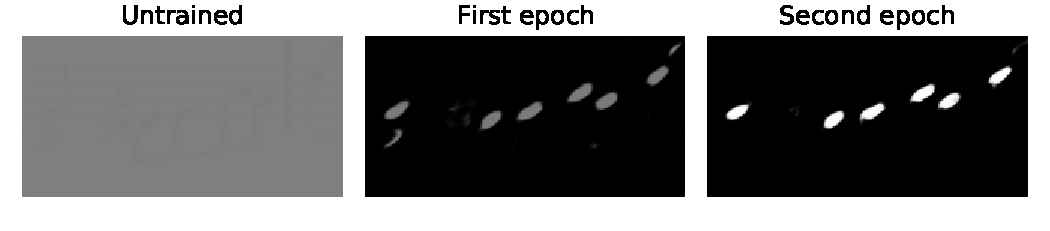
\includegraphics[width=140mm]{../../figures/03-activation-function/progression.pdf}
    \caption{The training process starts by learning to output a mostly black image, which probably causes the model to overshoot during the fully-supervised training and get stuck in the "dying ReLU" problem.}
    \label{fig:ActivationTrainingProgression}
\end{figure}

Interestingly enough, this problem happens only when training in the fully-supervised mode. We have never encountered it, when training in the semi-supervised mode. This again suggests that the unlabeled data acts as regularization, damping any extreme gradients, and stabilizing the training.

We also tried using the leaky ReLU function [CITE] with parameter $\alpha = 0.01$, however the problem still remained. Maybe a larger value for $\alpha$ would help, although we already knew that ELU works, so we haven't explored this further.

\begin{figure}[ht]
    \centering
    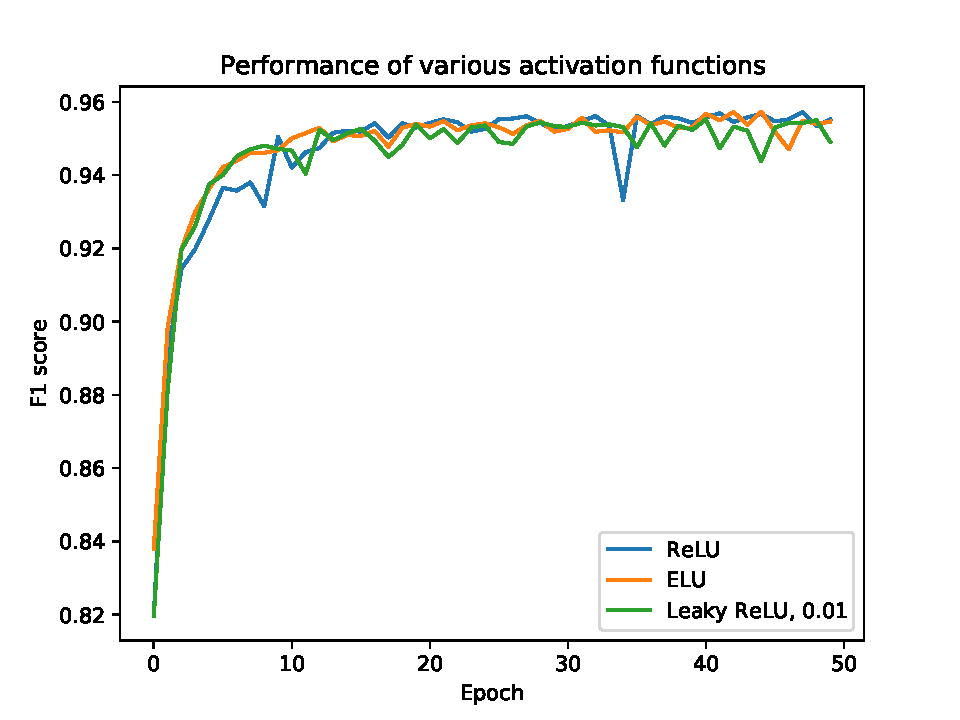
\includegraphics[width=140mm]{../../figures/03-activation-function/performance.pdf}
    \caption{An experiment from section \ref{sec:UtilizingCvcMuscima} with 8 inner features, trained in fully-supervised mode with various activation functions. All runs show the same performance.}
    \label{fig:ActivationFunctionPerformances}
\end{figure}

We run one of the experiments from section \ref{sec:UtilizingCvcMuscima} with all proposed activation functions to see what impact it has on model performance (figure \ref{fig:ActivationFunctionPerformances}). We can clearly see that they all perform equally well, so we choose ELU as the only activation function that does not suffer from the convergence problem. We thereby validate the work of Dorfer. et al. [CITE] (their article does not provide explanation for the use of ELU, but we belive they must have encountered these exact same problems).
